% Jaring-jaring kubus: susunan salib (1-4-1), tangga (2-2-2), dan 3-3 — semuanya jaring sah
% Kompilasi: pdflatex jaring-jaring-kubus-tikz.tex
\documentclass[tikz,border=10pt]{standalone}
\usepackage{amsmath}
\definecolor{bgdark}{HTML}{171D2B}
\definecolor{akun}{HTML}{F7B538}
\begin{document}
\pagecolor{bgdark}
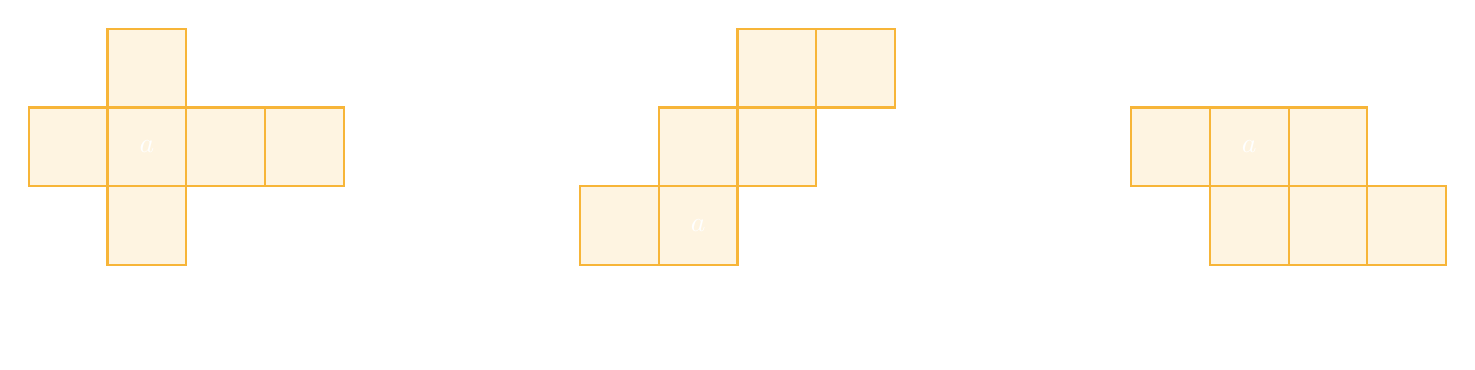
\begin{tikzpicture}[scale=1.0, text=white, font=\sffamily]
  % ---- Susunan salib (1-4-1, kiri) ----
  \begin{scope}[shift={(0,0)}]
    \foreach \x/\y in {0/1, 1/1, 2/1, 3/1, 1/2, 1/0}{
      \draw[akun, thick, fill=akun!15] (\x,\y) rectangle ++(1,1);
    }
    \node[text=white] at (1.5,1.5) {$a$};
    \node[text=white, font=\sffamily\small] at (2,-0.7) {Salib (1-4-1)};
  \end{scope}
  % ---- Susunan tangga (2-2-2, tengah) ----
  \begin{scope}[shift={(7,0)}]
    \foreach \x/\y in {0/0, 1/0, 1/1, 2/1, 2/2, 3/2}{
      \draw[akun, thick, fill=akun!15] (\x,\y) rectangle ++(1,1);
    }
    \node[text=white] at (1.5,0.5) {$a$};
    \node[text=white, font=\sffamily\small] at (2,-0.7) {Tangga (2-2-2)};
  \end{scope}
  % ---- Susunan 3-3 (kanan) ----
  \begin{scope}[shift={(14,0)}]
    \foreach \x/\y in {0/1, 1/1, 2/1, 1/0, 2/0, 3/0}{
      \draw[akun, thick, fill=akun!15] (\x,\y) rectangle ++(1,1);
    }
    \node[text=white] at (1.5,1.5) {$a$};
    \node[text=white, font=\sffamily\small] at (2,-0.7) {Tiga-tiga (3-3)};
  \end{scope}
\end{tikzpicture}
\end{document}
